%%%%%%%%%%%%%%%%%%%%%%%%%%%%%%%%%%%%%%%%%%%%%%%%%%%%%%%%%%%%%%%%%%%%%
%%                                                                 %%
%% Please do not use \input{...} to include other tex files.       %%
%% Submit your LaTeX manuscript as one .tex document.              %%
%%                                                                 %%
%% All additional figures and files should be attached             %%
%% separately and not embedded in the \TeX\ document itself.       %%
%%                                                                 %%
%%%%%%%%%%%%%%%%%%%%%%%%%%%%%%%%%%%%%%%%%%%%%%%%%%%%%%%%%%%%%%%%%%%%%

%%\documentclass[referee,sn-basic]{sn-jnl}% referee option is meant for double line spacing

%%=======================================================%%
%% to print line numbers in the margin use lineno option %%
%%=======================================================%%

%%\documentclass[lineno,sn-basic]{sn-jnl}% Basic Springer Nature Reference Style/Chemistry Reference Style

%%======================================================%%
%% to compile with pdflatex/xelatex use pdflatex option %%
%%======================================================%%

%%\documentclass[pdflatex,sn-basic]{sn-jnl}% Basic Springer Nature Reference Style/Chemistry Reference Style

%%\documentclass[sn-basic]{sn-jnl}% Basic Springer Nature Reference Style/Chemistry Reference Style
\documentclass[sn-mathphys]{sn-jnl}% Math and Physical Sciences Reference Style
%%\documentclass[sn-aps]{sn-jnl}% American Physical Society (APS) Reference Style
%%\documentclass[sn-vancouver]{sn-jnl}% Vancouver Reference Style
%%\documentclass[sn-apa]{sn-jnl}% APA Reference Style
%%\documentclass[sn-chicago]{sn-jnl}% Chicago-based Humanities Reference Style
%%\documentclass[sn-standardnature]{sn-jnl}% Standard Nature Portfolio Reference Style
%%\documentclass[default]{sn-jnl}% Default
%%\documentclass[default,iicol]{sn-jnl}% Default with double column layout

%%%% Standard Packages
%%<additional latex packages if required can be included here>
%%%%

%%%%%=============================================================================%%%%
%%%%  Remarks: This template is provided to aid authors with the preparation
%%%%  of original research articles intended for submission to journals published 
%%%%  by Springer Nature. The guidance has been prepared in partnership with 
%%%%  production teams to conform to Springer Nature technical requirements. 
%%%%  Editorial and presentation requirements differ among journal portfolios and 
%%%%  research disciplines. You may find sections in this template are irrelevant 
%%%%  to your work and are empowered to omit any such section if allowed by the 
%%%%  journal you intend to submit to. The submission guidelines and policies 
%%%%  of the journal take precedence. A detailed User Manual is available in the 
%%%%  template package for technical guidance.
%%%%%=============================================================================%%%%

\jyear{2021}%

%% as per the requirement new theorem styles can be included as shown below
\theoremstyle{thmstyleone}%
\newtheorem{theorem}{Theorem}%  meant for continuous numbers
%%\newtheorem{theorem}{Theorem}[section]% meant for sectionwise numbers
%% optional argument [theorem] produces theorem numbering sequence instead of independent numbers for Proposition
\newtheorem{proposition}[theorem]{Proposition}% 
%%\newtheorem{proposition}{Proposition}% to get separate numbers for theorem and proposition etc.

\theoremstyle{thmstyletwo}%
\newtheorem{example}{Example}%
\newtheorem{remark}{Remark}%

\theoremstyle{thmstylethree}%
\newtheorem{definition}{Definition}%

\raggedbottom
%%\unnumbered% uncomment this for unnumbered level heads

\begin{document}

\title[Article Title]{Tie-deletion can prevent polarization}
\subtitle{Co-evolution of opinion and network dynamics}

%%=============================================================%%
%% Prefix	-> \pfx{Dr}
%% GivenName	-> \fnm{Joergen W.}
%% Particle	-> \spfx{van der} -> surname prefix
%% FamilyName	-> \sur{Ploeg}
%% Suffix	-> \sfx{IV}
%% NatureName	-> \tanm{Poet Laureate} -> Title after name
%% Degrees	-> \dgr{MSc, PhD}
%% \author*[1,2]{\pfx{Dr} \fnm{Joergen W.} \spfx{van der} \sur{Ploeg} \sfx{IV} \tanm{Poet Laureate} 
%%                 \dgr{MSc, PhD}}\email{iauthor@gmail.com}
%%=============================================================%%

\author*[1,2]{\fnm{Mikkel} \sur{Werling}}\email{werling1407@gmail.com}

\author[2,3]{\fnm{Paul} \sur{Smaldino}}\email{iiauthor@gmail.com}
\equalcont{These authors contributed equally to this work.}

\author[1,2]{\fnm{Riccardo} \sur{Fusaroli}}\email{iiiauthor@gmail.com}
\equalcont{These authors contributed equally to this work.}

\affil*[1]{\orgdiv{Department}, \orgname{Organization}, \orgaddress{\street{Street}, \city{City}, \postcode{100190}, \state{State}, \country{Country}}}

\affil[2]{\orgdiv{Department}, \orgname{Organization}, \orgaddress{\street{Street}, \city{City}, \postcode{10587}, \state{State}, \country{Country}}}

\affil[3]{\orgdiv{Department}, \orgname{Organization}, \orgaddress{\street{Street}, \city{City}, \postcode{610101}, \state{State}, \country{Country}}}

%%==================================%%
%% sample for unstructured abstract %%
%%==================================%%

\abstract{
    Discovering what conditions can prevent political polarization is a vital and pressing issue, as political polarization can critically harm democratic institutions \cite{boxell_cross-country_2020, levin_dynamics_2021}. Identifying the conditions that can lead a system to polarization is a primary interest for the scientific field of opinion dynamics \cite{flache_models_2017}. Previous models of opinion dynamics have largely neglected the co-evolution of opinion and network dynamics \cite{flache_models_2017, galesic_integrating_2021}. This is despite the fact that the two dynamics are known to be interacting processes \cite{bener_empirical_2016, mcpherson_birds_2001, kossinets_origins_2009}.
  Moreover, the field of opinion dynamics suffers from not being able to incorporate empirical data in its theoretical models, which severely limits the field's ability to make reliable explanations and predictions \cite{flache_models_2017,galesic_integrating_2021, mas2019challenges}.
  This thesis tries to fill both of these gaps in the literature by developing a co-evolutionary agent-based model of opinion and network dynamics. Cutting-edge techniques of hyperparameter optimization are used to investigate how well the patterns of generated networks correspond to the patterns of seven empirical social networks. This thesis expands upon previous uses of hyperparameter optimization for agent-based modeling by calculating the importance of the model parameters using a functional analysis of variance (fANOVA).
  The results show that triadic closure can explain the patterns of empirical networks better than the most used network generating algorithms. Moreover, when the empirical social networks are large and highly opinionated, co-evolutionary models offer much better explanations than models that do not include opinion dynamics.
  Contrary to recent findings \cite{sasahara_social_2021}, the main result of this thesis is that avoiding polarization can be facilitated by the deletion of ties between dissimilar agents. This thesis offers novel perspectives on possible remedies for polarization, and improves upon the ability of previous models to explain how social networks are created. }

%%================================%%
%% Sample for structured abstract %%
%%================================%%

% \abstract{\textbf{Purpose:} The abstract serves both as a general introduction to the topic and as a brief, non-technical summary of the main results and their implications. The abstract must not include subheadings (unless expressly permitted in the journal's Instructions to Authors), equations or citations. As a guide the abstract should not exceed 200 words. Most journals do not set a hard limit however authors are advised to check the author instructions for the journal they are submitting to.
% 
% \textbf{Methods:} The abstract serves both as a general introduction to the topic and as a brief, non-technical summary of the main results and their implications. The abstract must not include subheadings (unless expressly permitted in the journal's Instructions to Authors), equations or citations. As a guide the abstract should not exceed 200 words. Most journals do not set a hard limit however authors are advised to check the author instructions for the journal they are submitting to.
% 
% \textbf{Results:} The abstract serves both as a general introduction to the topic and as a brief, non-technical summary of the main results and their implications. The abstract must not include subheadings (unless expressly permitted in the journal's Instructions to Authors), equations or citations. As a guide the abstract should not exceed 200 words. Most journals do not set a hard limit however authors are advised to check the author instructions for the journal they are submitting to.
% 
% \textbf{Conclusion:} The abstract serves both as a general introduction to the topic and as a brief, non-technical summary of the main results and their implications. The abstract must not include subheadings (unless expressly permitted in the journal's Instructions to Authors), equations or citations. As a guide the abstract should not exceed 200 words. Most journals do not set a hard limit however authors are advised to check the author instructions for the journal they are submitting to.}

\keywords{agent-based modeling, opinion dynamics, social influence, co-evolution, social networks}

%%\pacs[JEL Classification]{D8, H51}

%%\pacs[MSC Classification]{35A01, 65L10, 65L12, 65L20, 65L70}

\maketitle

\section{Introduction}
\label{introduction}
Democracies around the world are experiencing increased amounts of political polarization \cite{boxell_cross-country_2020,mccoy_polarization_2018, somer_deja_2018}. 
As a result, cooperating with other people becomes harder, which can severely damage the ability of democratic systems to solve problems \cite{andris_rise_2015,levin_dynamics_2021,mccoy_polarization_2018}. 
A striking recent example is the uniquely severe rise of polarization in the political system of the United States \cite{dimock_america_2020}. 
During the last two decades, the amount of overlap of opinions between the two political parties has decreased substantially, which has led to gridlock, government shutdowns, and failure to enact new legislation (see Figure~\ref{fig:house_of_reps}) \cite{andris_rise_2015, pew_research_center_political_2014-1}. The cost of polarization was seen most severely by the fact that the global COVID-19 pandemic failed to generate a common effort from the two parties. Instead, preventative measures such as masks became party crests \cite{macy2021polarization}.

A related concept to political polarization is affective polarization. Affective polarization refers to the extent which citizens experience negative feelings for political parties other than their own \cite{boxell_cross-country_2020, iyengar_origins_2019}. 
Once again, the United States is reported to have uniquely high amounts of affective polarization \cite{boxell_cross-country_2020}. 
Although the United States is unique in the extent of affective polarization, countries such as France, Switzerland, and Denmark have also had increased levels of affective polarization in the last two decades \cite{boxell_cross-country_2020}. 
The increase in polarization is in other words a general and global trend \cite{mccoy_polarization_2018, somer_deja_2018, wilson_polarization_2020}. 
With that said, the polarization of opinions does not seem to be an inevitable state for democracies. 
During the last two decades, European democracies such as Sweden, Norway, and Germany have experienced higher degrees of consensus and a decrease in affective polarization \cite{boxell_cross-country_2020}. 

\noindent Despite the decrease in affective polarization in certain northern European countries, polarization globally is on the rise \cite{boxell_cross-country_2020,mccoy_polarization_2018, somer_deja_2018}. There is reason to believe that the general problem of polarization might be getting worse due to technological advances.
Specifically, a growing literature has reported that information is not distributed uniformly across the users of the internet and social media \cite{taylor_exploring_2018, sasahara_social_2021,baumann_modeling_2020,tsai_echo_2020}. Instead, information is being catered to the individual based on their previous search history and behavior on social media \cite{geschke2019triple}. Very different people will therefore be shown very different pieces of information, as users are only presented with a small subset of the available information. 
Heavily influenced by confirmation bias, this can lead to circumstances where almost all opinions one is exposed to are congruent with one’s prior beliefs \cite{baumann_modeling_2020}. Such circumstances are popularized under the term echo chambers on social media. Echo chambers are often cited as one of the main reasons for the increase in political polarization \cite{baumann_modeling_2020, sasahara_social_2021, tsai_echo_2020, geschke2019triple}. 

Because of technology's impact on the level of polarization, the internet has been called a mixed blessing \cite{lev-on_happy_2009}. On the one hand, individuals can access more diverse information via the internet, which can help decrease polarization. On the other hand, the internet also enables encounters of extremely opposing opinions by chance, which can increase polarization \cite{lev-on_happy_2009}.
Previous work paints a murky picture concerning the effect of being presented with very different opinions. The work of \citeA{levy_social_2021} suggests that when people are presented with a diverse set of views, they generally tend to have fewer negative feelings towards other political parties than their own. This result seems to go against the study of \citeA{bail_exposure_2018}, where exposure to directly opposing views can cause opinions to become more polarized than they were before exposure. 
On a similar note, higher involvement in one’s echo chamber correlates with more with emotions of negative valence, which suggests that echo chambers are driven largely by outrage. In other words, the most active users in an echo chamber are the ones who are most displeased with the opinions of people outside their echo chamber \cite{del_vicario_echo_2016}.

\noindent Although polarization is usually described in the context of political polarization, polarization is not necessarily a political phenomenon. In fact, polarization can critically impair any social system's ability to cooperate successfully \cite{levin_dynamics_2021}. It is therefore vital to identify and understand what mechanisms can lead a system to polarization, consensus, or anywhere in between the two extremes. This is no easy task. Opinion formation and opinion dynamics are highly complex phenomena \cite{baumann2021modeling}. 
Despite the complexity of the problem, an entire scientific field has been dedicated to the study of how opinions change. The study of the dynamics shaping opinions is aptly named opinion dynamics. Formal models of opinion dynamics often neglect the fact that agents can not only change their opinions but also change their peers \cite{flache_models_2017}. The models of opinion dynamics typically assume a static network structure in which agents are situated \cite{galesic_integrating_2021}. By doing so, these models fail to take into account that social networks are dynamic and that the structure of the networks is likely co-evolving with opinions \cite{de2022modelling,galesic_integrating_2021}. The interdependence between the dynamics of social networks and opinion dynamics is largely understudied, despite the fact that the two processes are highly interacting \cite{asikainen_cumulative_2020,bruch_agent-based_2015,galesic_integrating_2021,kossinets_origins_2009,noorazar_classical_2020}. It is therefore not surprising that the dynamic relationship between the two dynamics has often been reported as an important avenue for future research \cite{flache_models_2017,galesic_integrating_2021}. 

\noindent Another important avenue to gain insights into is how to incorporate empirical data in theoretical models \cite{mas2019challenges}. This is an especially pertinent problem in the field of opinion dynamics, which often fails to account for how the results of their models match empirical data \cite{galesic_integrating_2021,flache_models_2017, mas2019challenges}. 
The lack of empirical integration is understandable, as opinions are notoriously hard to measure \cite{mas2019challenges}. Moreover, most of the models of opinion dynamics are not meant to accurately predict how opinions evolve over time, but rather point out interesting interactions between key variables in formal models \cite{mas2019challenges}. Such theoretical models are useful for theory building, but they often run the risk of being too detached from the real world to be useful \cite{smaldino_how_2020, mas2019challenges}.  

\noindent This thesis seeks to fill these two critical gaps in the current literature on opinion dynamics: the need to integrate both empirical data and the co-evolution of networks and opinion dynamics. This thesis is organized into four parts. The introduction provides an overview of previous methods and vital mechanisms to consider. This is done by first explaining how agent-based models are well-equipped to investigate complex systems. Next, the critical underlying mechanisms of opinion and network dynamics are identified and introduced. A co-evolutionary agent-based model of opinion and network dynamics is built on the basis of these mechanisms, drawing on insights from data science, social psychology, computational biology, and network science. The model is specifically designed to help illuminate the co-evolution of opinion and network dynamics. 
The second part of the thesis integrates empirical data into the agent-based modeling process by investigating how well the agent-based model can generate the patterns found in real-world networks. To do so, cutting-edge techniques of hyperparameter optimization are employed. This thesis expands upon previous use of this technique in agent-based modeling by also implementing a functional analysis of variance (fANOVA) of the hyperparameter importance \cite{hutter2014efficient}. 
The third part of this thesis is focused on how co-evolution impacts opinion dynamics. It does so by exploring how the polarization of the system is influenced by the model parameters. This section focuses on understanding how tie-deletion to dissimilar individuals might prevent polarization. 
Finally, the fourth part of the paper discusses the overall findings and presents the key limitations of the model. 

\section{Agent-based modeling of complex phenomena}
The social sciences face the daunting task of trying to explain and predict the behavior of extremely complex systems. 
Historically, social scientists have explained such systems by relying on the power of language using verbal models \cite{smaldino_how_2020}. Verbal models typically explain a system by providing useful analogies, which can help illuminate the system of interest. These analogies are often ambiguous and several interpretations of the same model are possible. The benefit of this ambiguity is that verbal models often incorporate many realistic social and cognitive mechanisms \cite{fogarty_ten_2022}. But ambiguity is often something to be avoided in science, as clarity and precision are necessities for developing useful theories of reality \cite{smaldino_how_2020}. 
Formal models offer an alternative to verbal models, as they offer the kind of precision that is lacking in verbal models at the cost of some realism. Typical examples of formal models are mathematical models, where different variables describe forces in the system \cite{fogarty_ten_2022}. Formal models are especially hard to build for complex systems as the different constituents of the system are hard to reduce to single components \cite{smaldino_how_2020, poli2013note}. Formal models of complex systems often solve this problem by making simplifying assumptions, which reduces the realism of the models \cite{fogarty_ten_2022}. 

Agent-based models are well-equipped to strike a balance between the precision of formal models and the realism of verbal models \cite{flache_between_2018,galesic_integrating_2021,epstein1999agent,mas2014cultural}. This is done by investigating the macro-behaviors of a system, where the micro-behaviors are specified \cite{bruch_agent-based_2015,epstein1999agent,flache_between_2018}. In particular, agent-based models are well-suited when analyzing systems where more is known about interactions between individuals instead of interactions between variables \cite{geschke2019triple}. As is the case with any model, the results critically hinge on the assumptions of the model. It is the role of the modeler to provide as empirically plausible mechanisms as possible for the system of study \cite{crooks2012introduction,epstein1999agent,page2010diversity}. At the same time, the value of a model comes from the fact that it is a simplification of reality. The model should be as simple as it can be and as complicated as it needs to be in order to answer its questions \cite{smaldino_how_2020}. The hope is that by simplifying the system to a sufficient extent, we can observe and understand some important features of even extremely complex systems \cite{fogarty_ten_2022,smaldino_models_2016, smaldino_how_2020, smaldino_models_2022}.

\noindent One of the complex systems that the social sciences have studied for decades is the dynamics governing how opinions are formed and changed \cite{flache_models_2017}. Describing the mechanisms which shape opinion dynamics constitutes a complex problem \cite{mas2019challenges}, in the sense that opinion dynamics is governed by multiple interacting systems. 
How opinions are changed is both the result of how people update their beliefs cognitively and how they are exposed to different perspectives socially \cite{friedkin_social_1990,spears_social_2021}. 

\section{Central Mechanisms}
Investigating the complex system of opinion dynamics is the main aim of this paper. In the following sections, the central mechanisms of opinion dynamics are introduced. The specific focus will be on the tendency for similar individuals to cluster together and on how social relations influence the individual's opinion. 

\subsection{Homophily}
One of the most robust findings of the social world is summed up in the famous phrase "birds of a feather flock together" \cite{mcpherson_birds_2001}. This phrase refers to the fact that assortment in humans is non-random, and is often based on how similar individuals are \cite{asikainen_cumulative_2020,crandall_feedback_2008,mcpherson_birds_2001}. The observation that similarity breeds social connections is called observed homophily \cite{mcpherson_birds_2001,kossinets_origins_2009}. In all types of human social networks, observed homophily seems ubiquitous.
For all demographic variables which have been investigated, including gender, race, religion, and socioeconomic class, there is always a tendency for more similar individuals to cluster together \cite{asikainen_cumulative_2020,mcpherson_birds_2001, taylor_exploring_2018}. 

\noindent Observed homophily has mainly been explained using a psychological and a structural explanation. The psychological explanation seeks to explain observed homophily by the fact that people seem to exhibit a psychological preference to be with people like themselves. This psychological preference is referred to as choice homophily \cite{asikainen_cumulative_2020,mcpherson_birds_2001,winter_you_2020}.
Such a preference might have evolved as interacting with similar people ensures easier communication and enhances the individual’s ability to predict the other person’s behavior \cite{kossinets_origins_2009,winter_you_2020}. In this sense, assortment based on similarity could have evolved to facilitate cooperation, because coordination between similar individuals is simpler and less costly for the individual \cite{winter_you_2020,carter2015phenotypic, smaldino2019social}. 

Although choice homophily seems to be an important piece of the puzzle, observed homophily could also be explained by structural constraints. Such constraints could limit how dissimilar choices of interactions are available \cite{peixoto_disentangling_2022}. As an example, if you work as a female nurse, chances are that most of your interactions at work will be with other females. 
In this case, even if you do not have a strong psychological preference for interacting with people like yourself, the social interactions available to you might primarily be with people similar to you. 
The existing assortment in the network makes the probability of interacting with similar individuals much higher than with non-similar individuals \cite{peixoto_disentangling_2022}. Such structural factors contributing to high levels of observed homophily are referred to as structural homophily \cite{asikainen_cumulative_2020,mcpherson_birds_2001,winter_you_2020}. 

\noindent Observed homophily hints at the prevalent intuition that you have more in common with your friends than you have with strangers \cite{mcpherson_birds_2001}.
Despite its prevalence, few studies have been made to gauge how homophily influences social relations. One such study was made by \citeA{kossinets_origins_2009}, which investigated how observed homophily manifested in real dynamical social networks. They recorded social interactions at a large university for a year. These interactions allowed \citeA{kossinets_origins_2009} to estimate not only how social ties changed over time, but also how similar individuals of the social networks were. Their findings are of significant importance to this thesis. First, the results confirm what one might intuitively expect - you have more in common with your friends than you have with strangers. But their findings suggest that this is a special case of a more general phenomenon; that distance in similarity is a function of distance in the social network (see Figure~\ref{fig:distance_similarity}). The further you are removed from someone in the social network, the less you will have in common \cite{kossinets_origins_2009}. 
The connection between distance in similarity and distance in the social network is a robust finding which has also been shown in other large empirical studies \cite{bener_empirical_2016,crandall_feedback_2008}.

\noindent Choice and structural homophily are normally used as separate explanations for the observed homophily in social networks, but they are not mutually exclusive. Rather, it seems that the two processes can facilitate each other \cite{asikainen_cumulative_2020}. For instance, even low amounts of choice homophily could evolve into structural homophily over time \cite{asikainen_cumulative_2020,kossinets_origins_2009,taylor_exploring_2018}. When even a few distant similar individuals connect because of choice homophily, the correlation between proximity and similarity increases. As such, even small preferences will add up over time, and make the correlation between proximity and similarity stronger and stronger, which will lead to increased structural homophily \cite{kossinets_origins_2009}. 
Both structural and choice homophily contribute to the link between distance in similarity and distance in social networks \cite{bener_empirical_2016}. Structural homophily plays a large role as new ties are primarily made to people close to you in the social network \cite{bianconi_triadic_2014, peixoto_disentangling_2022}. When similarity and distance in social networks are connected, structural homophily will increase the observed homophily of the system. Controlling for both distance in the network and shared social circles, generating new social ties is more likely between similar agents \cite{kossinets_origins_2009, bener_empirical_2016}.

\noindent Similarity is not only predictive of which new social ties will be created but also which old ties will be deleted. Although homophily has almost exclusively been studied as a process that makes similar individuals more likely to generate new ties to each other \cite{noel2011unfriending, bener_empirical_2016}, homophily has been shown empirically to also play a key role in tie-deletion. More similar individuals have more stable connections, with a lower propensity to delete ties over time \cite{noel2011unfriending, bener_empirical_2016, mcpherson_birds_2001, kossinets_origins_2009}.
In addition to choice and structural homophily, the connection between similarity and distance is also driven by the increased propensity to delete ties to dissimilar people \cite{kossinets_origins_2009, bener_empirical_2016}. The effect becomes more extreme as interactions between peers tend to make like-minded individuals even more like-minded \cite{friedkin_social_1990, spears_social_2021}. Complementing the empirical studies on tie-deletion, the famous computational work of \citeA{schelling1971dynamic} shows that including even subtle tendencies of tie-deletion of dissimilar pairs can create global patterns of network segregation and community structures that are characteristic of many real-world social networks. 

\subsection{Social Influence}
Humans are inherently a social species \cite{kurzban2015evolution}. We do not think and form our opinions in a vacuum. Either via social media, debates, or discussions with friends, opinions are constantly being shared, debated, and discussed with other individuals. 
As a result of these social interactions, the opinions of the people involved in the interaction might change. 
The influence that social encounters and social relations have on the opinions of the involved agents is referred to as social influence \cite{friedkin_social_1990}. Social influence has been proposed as the most important effect in shaping an individual’s opinions \cite{chacoma_opinion_2015, flache_between_2018}. As was the case in the previous section, the similarity of individuals is central to how social relations influence opinions. When similar individuals interact, their opinions typically become more similar than they were before interactions \cite{takacs_discrepancy_2016}. On the other hand, dissimilar individuals can repulse each other, which can cause opinions to become more dissimilar from each other than they were initially \cite{hilmert2006positive, cikara2014neuroscience}.  

In this thesis, we will distinguish between positive and negative social influence. Positive social influence refers to the force which drives similar individuals to become more similar through interactions \cite{flache_models_2017,levin_dynamics_2021}. 
This can be thought of as instances of reaching a compromise, finding common ground, or seeing the other person’s perspective on a topic. Interactions that are driven by positive social influence will be referred to as positive interactions in this thesis. Negative social influence refers to the force which causes dissimilar agents to become more dissimilar as a result of interactions \cite{flache_models_2017}. 
Examples include moral outrage or out-group aversion. Interactions that are driven by negative social influence will be referred to as negative interactions in this thesis. It is important to note that although positive influence seems to be a robust empirical finding, negative influence is more elusive \cite{flache_models_2017,takacs_is_2014,turner_paths_2018}. 
With that said, there is evidence that suggests that exposure to opposing views can lead to increased polarization \cite{bail_exposure_2018, hilmert2006positive, cikara2014neuroscience}.

\section{Opinion Dynamics}
The field of opinion dynamics attempts to identify key mechanisms which shape how opinions change over time using formal and agent-based models \cite{flache_models_2017,flache_between_2018,noorazar_classical_2020}. Two of the most robustly identified mechanisms are social influence and homophily \cite{flache_models_2017}. The models from opinion dynamics are often analogous, drawing inspiration from statistical physics in the structure and mechanisms of their scientific models \cite{galesic_integrating_2021}. Both continuous and discrete opinions have previously been studied, as well as systems where agents have multiple opinions of interest \cite{flache_models_2017}. The standard approach in opinion dynamics is to use empirical studies of psychological and sociological mechanisms to inform the assumptions of their theoretical models. These models are typically used to identify how these empirically justified parameters interact with each other  \cite{baumann2021modeling,chacoma_opinion_2015,flache_models_2017,friedkin_social_1990,noorazar_classical_2020,spears_social_2021,turner_paths_2018}. 

\subsection{Dynamical networks}
By modeling opinion dynamical systems in computational models, researchers in opinion dynamics create simple systems which represent the more complex and messy real social world. These simplified systems are normally studied to identify which conditions can give rise to polarization or consensus in terms of the opinions of simulated agents \cite{flache_models_2017}. As has already been alluded to in the \textit{\nameref{introduction}}, previous models have focused on social influence without considering how the social interactions change as a result of changes in opinions \cite{galesic_integrating_2021,holme_nonequilibrium_2006,jalili_coevolution_2015}. Central to most classical models of opinion dynamics is that agents are situated in static, theoretical networks \cite{flache_models_2017}. The assumption of static networks is consequential. Real social networks are inherently dynamic, with new ties being formed and deleted over time. As has already been established, empirical work suggests that the processes of opinion and network dynamics are largely interdependent. New social interactions are more likely between similar agents, and tie deletion is more likely between dissimilar agents \cite{kossinets_origins_2009, bener_empirical_2016}. Additionally, it is worth noting that when computational models of static networks include negative social influence, the system cannot overcome polarization of opinions \cite{flache_models_2017, kozma2008consensus}. Previous work has already highlighted how important the assumption of static networks is. Using the mechanism of deleting ties to dissimilar agents, \citeA{kozma2008consensus} shows that co-evolution can create clusters of like-minded individuals which has a large impact on the convergence time of reaching consensus \cite{kozma2008consensus}. 
Although all models do some violence to the world by making assumptions, models should try to include the vital mechanisms of the system they are representing, while simplifying the system enough to understand it \cite{epstein1999agent,smaldino_models_2016}. It is one of this thesis's most central claims that the co-evolution of network and opinion dynamics should be considered a vital mechanism. To better explain how opinions are shaped over time, we need to include not only the basic underlying mechanisms of social influence but also network dynamics. 

\section{Network Dynamics}
Models of opinion dynamics typically situate the agents of their models in static, theoretical networks \cite{flache_models_2017, galesic_integrating_2021}. Classic examples of the networks used in most models of opinion dynamics include ring lattices, small-world networks and scale-free networks \cite{barabasi_scale-free_2003,watts_collective_1998}. Both small-world and scale-free networks are famous for being able to capture essential features of real social networks. Small-world networks are able to capture the general tendency of high average clustering coefficient and low average path length found in most social networks \cite{watts_collective_1998}. This is achieved by starting with a ring lattice and rewiring a small percentage of the ties randomly. Randomly rewiring a few ties creates highways of information which decreases the average path length considerably \cite{watts_collective_1998}. Scale-free networks can capture the general tendency of long tails in the degree distributions of social networks. The degree distribution of social networks often follows a power law, where a few nodes have an extremely high amount of edges, while most nodes only have a few \cite{barabasi_scale-free_2003}. Recent work calls into question how universal power laws are in empirical social networks and finds instead that most degree distributions from social networks follow a log-normal distribution \cite{broido_scale-free_2019}. Note that neither of the most used theoretical networks can generate all the essential features of social networks \cite{jacksonsearch2004}. Small-world networks have unrealistic degree distributions, and scale-free networks have very low average clustering coefficients. 

\subsection{Triadic Closure}
An alternative to the preferential attachment of scale-free networks and the rewiring of small-world networks is to consider what mechanisms govern how real social networks change over time. Both scale-free and small-world networks attempt to answer the question of how network characteristics could be generated, not why social networks have the characteristics that they do \cite{jacksonsearch2004}. An attempt at answering the why-question is the work by \citeA{jacksonsearch2004}, which emphasizes the role of triadic closure in network generation. Triadic closure refers to making new connections by generating new ties to "friends of friends", i.e. the edges of one's edges (see Figure~\ref{fig:tie_closure}). Reliably, triadic closure is found to be the most important and robust mechanism for how new connections are made in social networks \cite{asikainen_cumulative_2020,bianconi_triadic_2014,kossinets_origins_2009,peixoto_disentangling_2022}. Empirical studies on dynamical networks find that the probability of creating a new tie is a decreasing function of the distance in the network \cite{bener_empirical_2016,kossinets_origins_2009}. The less separated you are from someone, the more likely you are to form a social tie with this person. A popular colloquial framing for distance in social networks is to measure distance between individuals in "handshakes" \cite{smith2005networks}. One's friends are one handshake away, friends of friends are two handshakes away and so on. The empirical studies suggest that when you are two rather than three handshakes away from someone, you are 30 times more likely to form a connection (see Figure~\ref{fig:tie_closure}). This increase in likelihood only becomes more extreme when the distance is increased. When you are two rather than five handshakes away from someone, you are 2.500 times more likely to form a connection \cite{kossinets_origins_2009}. 

\subsubsection{Triadic closure and network metrics}
Using triadic closure as the generating principle for network formation has shown great promise in explaining some key characteristics of social networks \cite{ilany_social_2016}. In previous formal models of network formation, this is implemented by making most new connections via triadic closure while letting a few connections be made at random \cite{ilany_social_2016,jacksonsearch2004,jacksonmeeting2007}. These models can generate the important characteristic findings in social networks of high average clustering coefficient, low average path length and log-normal degree distributions \cite{jacksonsearch2004,jacksonmeeting2007}. 

\noindent It is worthwhile to pause to understand why these network metrics are important and why triadic closure might generate patterns akin to those of empirical social networks. The average clustering coefficient is a measure of how connected local communities are in networks \cite{watts_collective_1998}. Social networks typically exhibit high average clustering coefficients, which is closely linked to the fact that social networks typically consist of a number of tight-knitted, well-connected local communities \cite{peixoto_disentangling_2022, newman_finding_2006, crandall_feedback_2008}. Models of triadic closure are likely to exhibit high average clustering coefficients, as triadic closure will increase the number of local links \cite{jacksonmeeting2007}. 

The average path length refers to the average length of the shortest path between any two nodes in a network \cite{watts_collective_1998}. The average path length is important for how fast information or contagious diseases can spread in a network \cite{cowan2004network}. Social networks typically have low average path lengths, where no individual is many handshakes away from being connected to another individual \cite{backstrom2012four}. The network formation models using triadic closure also have low average path lengths, benefiting from similar mechanisms of randomness as small-world networks to achieve low average path lengths \cite{jacksonmeeting2007,watts_collective_1998}. As mentioned, a small amount of randomness can create long-range connections, which decreases the average path length substantially \cite{watts_networks_1999}.  

Finally, the degree distribution is the distribution of the number of edges each agent has in a network. As mentioned, social networks typically have log-normal or scale-free degree distributions. In networks with such degree distributions, some nodes will have a very large degree, while most nodes will have a relatively low degree \cite{bianconi_triadic_2014}. These types of degree distributions are generated via triadic closure. The reason is that triadic closure is a mechanism where the probability of generating a new connection is proportional to how many connections a node already has. High degree nodes have more possibilities for being selected for via triadic closure simply because they have higher degrees \cite{jacksonmeeting2007}. Similarly, low degree nodes will have fewer connections that could generate new ties with them via triadic closure. This effect is similar to the mechanisms of preferential attachment in scale-free networks \cite{barabasi_scale-free_2003}.

\begin{figure}[H]
    \centering
    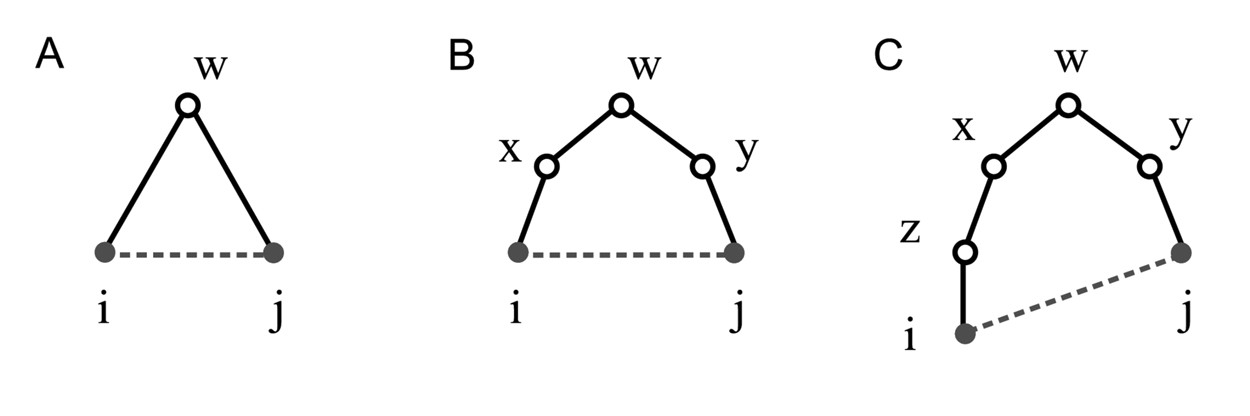
\includegraphics[width=.8\linewidth]{../plots/references/kossinets_watts.jpeg}
  \caption{Different types of tie closure. Taken from \protect\citeA{kossinets_origins_2009}. Panels show different ways of creating social ties via existing connections. Creating social ties in this way is often called tie-closure. Panel A depicts closing ties with a friend of a friend. This type of tie closure is called triadic closure. Panel B and C show longer cycles of closure.}
  \label{fig:tie_closure}
\end{figure}

\section{Co-evolution via tie-deletion}
Up until now, opinion and network dynamics have been presented and discussed in isolation. As mentioned, these dynamics are known to be interdependent \cite{bener_empirical_2016, kossinets_origins_2009, galesic_integrating_2021}.
It is easy to see how opinions could be influenced by network dynamics. 
As the social network changes, the available interactions for each agent will change. 
As one of the primary forces of opinion dynamics is social influence \cite{levin_dynamics_2021, chacoma_opinion_2015}, changes in the social network will have large effects on the opinions of the social agents of the network. 
As the social network already influences opinion dynamics, any mechanism that changes the ties in the network based on the opinions of the agents will cause opinion and network dynamics to co-evolve. 
There are good reasons to believe that such mechanisms are numerous \cite{bener_empirical_2016, kossinets_origins_2009, levin_dynamics_2021}.
In this thesis, the co-evolutionary mechanism considered will be the tie-deletion of dissimilar individuals. 
Tie deletion of dissimilar individuals has been shown empirically to be a robust phenomenon \cite{kossinets_origins_2009, bener_empirical_2016}. Moreover, this mechanism has been studied previously in similar models to the one presented in this thesis \cite{santos_cooperation_2006,sasahara_social_2021}. 
By using a tie-deletion as the co-evolutionary mechanism, this thesis can better assess the robustness of the current claims in the literature. 

\subsection{The effect of tie-deletions on cooperation}
The previous studies on how tie-deletion influences cooperation do not come exclusively from the field of opinion dynamics. For instance, the field of computational biology is especially keen on identifying what conditions must be satisfied to facilitate the evolution of cooperation. Computational biology should be considered an adjacent field to opinion dynamics, as they share much in their interests and in their methods \cite{dakin_dynamic_2018,melamed_strong_2016,pepper_mechanism_2002,santos_cooperation_2006, smaldino2019social}. 

\subsubsection{Tie-deletion facilitates cooperation}
\noindent In one of the studies from the field of computational biology, \citeA{santos_cooperation_2006} studied how social connections are linked to whether a system of agents can cooperate. Intuitively, one might expect that when a network of social actors becomes more connected, levels of cooperation in the system should increase. However, the opposite effect is observed. In their paper, \citeA{santos_cooperation_2006} consider agents playing game-theoretic games, where agents either cooperate or defect. 
\citeA{santos_cooperation_2006} analyze what happens when agents adjust their ties based on the interactions made with other agents. When cooperators interact with defectors, the social tie between cooperators and defectors has a chance of being rewired to a different agent. This keeps the number of edges constant but decreases how globally connected the network is \cite{santos_cooperation_2006}. Their results indicate that cooperation flourishes when the propensity for deleting ties between cooperators and defectors increases (see Figure~\ref{fig:santos}). The interpretation given by \citeA{santos_cooperation_2006} is that removing ties between cooperators and defectors increases positive assortment between cooperators and decreases positive assortment between defectors and cooperators. One of the striking attributes of this finding is that without any propensity for tie-deletion, cooperation does not evolve for conditions equivalent to the Prisoner’s Dilemma \cite{santos_cooperation_2006}. More generally, positive assortment has been found to be a robust facilitator of cooperation in computational biology \cite{boyd_coordinated_2010,dakin_dynamic_2018,melamed_strong_2016,pepper_mechanism_2002}. As an aside, \citeA{santos_cooperation_2006} also show that using even relatively simple principles of co-evolution, where network dynamics reflect the individual agent's reaction to their social interactions, can produce realistic social networks \cite{santos_cooperation_2006}. 

\begin{figure}[H]
    \centering
    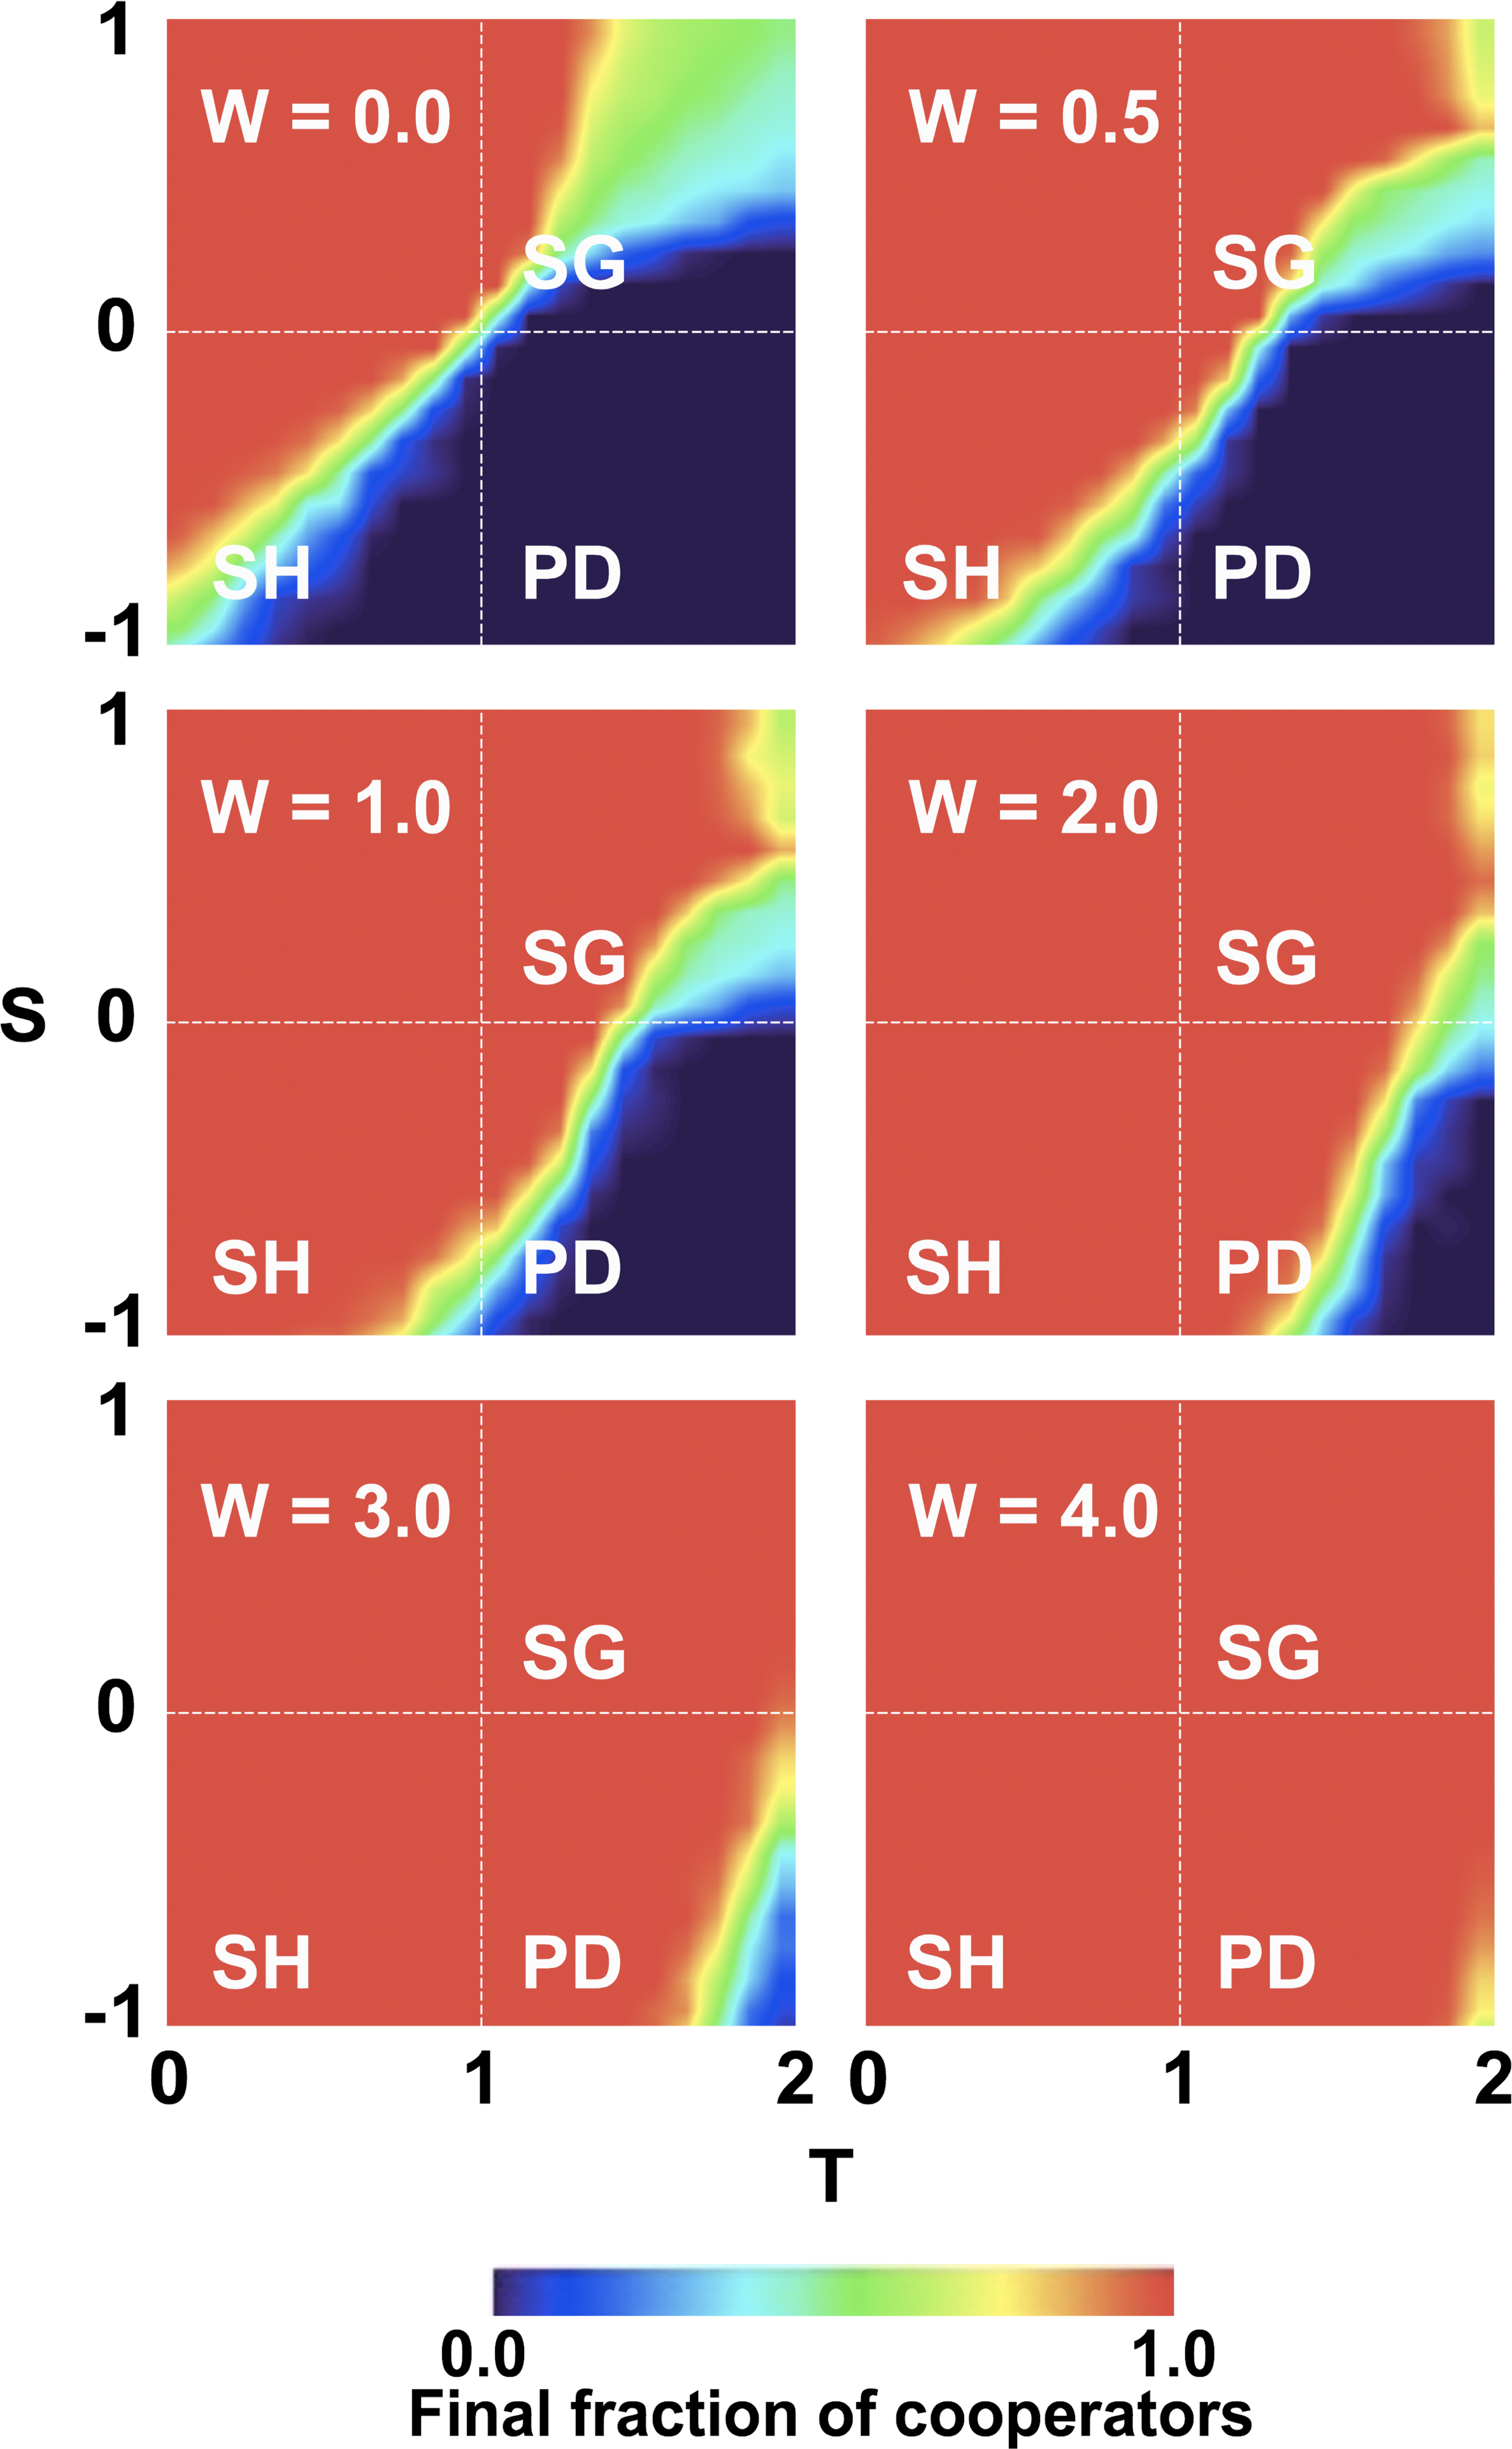
\includegraphics[width=.4\linewidth]{../plots/references/santos.png}
  \caption{Tie-deletions facilitate cooperation. Taken from \protect\citeA{santos_cooperation_2006}. Panels show simulations with different values of $W$. In the model of \protect\citeA{santos_cooperation_2006}, $W$ controls the propensity to delete ties between defectors and cooperators. Increases in $W$ lead to more rewiring of connections between defectors and cooperators. The y-axis shows the disadvantage of being cheated, and the x-axis shows the pay-off of cheating. The letters on the panel represent well-known game-theoretic dilemmas (Prisoners Dilemma, Stag Hunt, and Snow Drift Game). Colors show the final fraction of cooperators after simulations are completed. When $W = 4.0$, cooperators wipe out defectors. }
  \label{fig:santos}
\end{figure}

\subsubsection{Tie-deletion accelerates echo chambers}

\noindent Although the effect of positive assortment on cooperation seems general in the computational biology literature \cite{boyd_coordinated_2010,dakin_dynamic_2018,melamed_strong_2016,pepper_mechanism_2002}, some models from opinion dynamics point to an opposite result. When combined with social influence, \citeA{sasahara_social_2021} report that tie-deletion between dissimilar agents accelerates polarization by generating echo chambers that stifle cooperation (see Figure~\ref{fig:echo_chambers}). This is in line with the more intuitive explanation, where a decrease in communication between agents leads to a decrease in cooperation. Similarly, this is also in line with the research on echo chambers, where isolation leads to further polarization \cite{tsai_echo_2020, del_vicario_echo_2016}. 

\noindent It is noticeable that the same underlying mechanism can cause so drastically different results in the two models. For both studies, tie-deletion is a critical mechanism, but they find opposing directions of the effect \cite{santos_cooperation_2006,sasahara_social_2021}. It is precisely because of this dispute that further research should be made on how the deletion of negative ties can impact cooperation.

\begin{figure}[H]
    \centering
    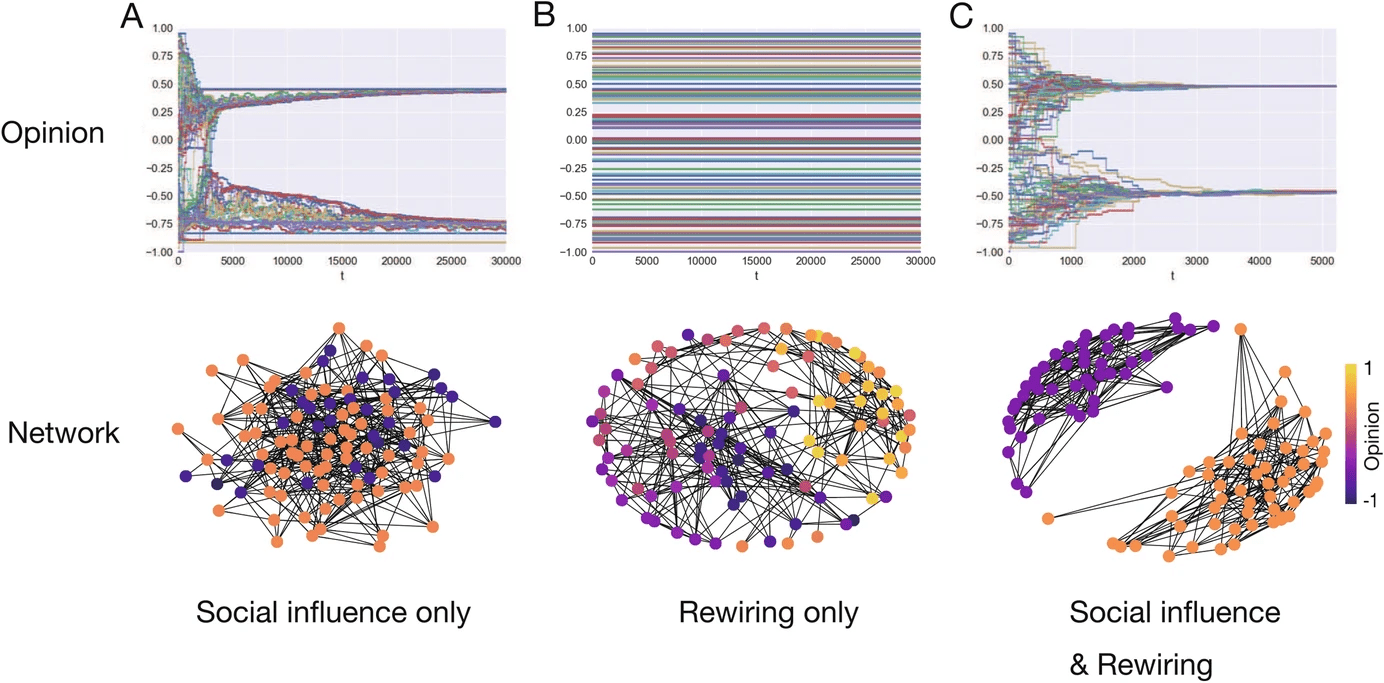
\includegraphics[width=.8\linewidth]{../plots/references/echo_chambers.png}
  \caption{Tie-deletion accelerates polarization. Taken from \protect\citeA{sasahara_social_2021}. The first row shows the trajectory of opinions over time and the second row shows the network after simulation. Columns show simulations of different conditions. Column A shows the results from only including social influence. Column B shows the results from conditions that only rewire connections based on opinions. Column C shows the results of including both social influence and rewiring. Of special interest is the last column, which shows that tie-deletion can accelerate echo chamber formation, as the opinions stabilize faster than when only social influence is included.}
  \label{fig:echo_chambers}
\end{figure}

\section{Results}\label{sec2}

Sample body text. Sample body text. Sample body text. Sample body text. Sample body text. Sample body text. Sample body text. Sample body text.

\section{This is an example for first level head---section head}\label{sec3}

\subsection{This is an example for second level head---subsection head}\label{subsec2}

\subsubsection{This is an example for third level head---subsubsection head}\label{subsubsec2}

Sample body text. Sample body text. Sample body text. Sample body text. Sample body text. Sample body text. Sample body text. Sample body text. 

\section{Equations}\label{sec4}

Equations in \LaTeX\ can either be inline or on-a-line by itself (``display equations''). For
inline equations use the \verb+$...$+ commands. E.g.: The equation
$H\psi = E \psi$ is written via the command \verb+$H \psi = E \psi$+.

For display equations (with auto generated equation numbers)
one can use the equation or align environments:
\begin{equation}
\|\tilde{X}(k)\|^2 \leq\frac{\sum\limits_{i=1}^{p}\left\|\tilde{Y}_i(k)\right\|^2+\sum\limits_{j=1}^{q}\left\|\tilde{Z}_j(k)\right\|^2 }{p+q}.\label{eq1}
\end{equation}
where,
\begin{align}
D_\mu &=  \partial_\mu - ig \frac{\lambda^a}{2} A^a_\mu \nonumber \\
F^a_{\mu\nu} &= \partial_\mu A^a_\nu - \partial_\nu A^a_\mu + g f^{abc} A^b_\mu A^a_\nu \label{eq2}
\end{align}
Notice the use of \verb+\nonumber+ in the align environment at the end
of each line, except the last, so as not to produce equation numbers on
lines where no equation numbers are required. The \verb+\label{}+ command
should only be used at the last line of an align environment where
\verb+\nonumber+ is not used.
\begin{equation}
Y_\infty = \left( \frac{m}{\textrm{GeV}} \right)^{-3}
    \left[ 1 + \frac{3 \ln(m/\textrm{GeV})}{15}
    + \frac{\ln(c_2/5)}{15} \right]
\end{equation}
The class file also supports the use of \verb+\mathbb{}+, \verb+\mathscr{}+ and
\verb+\mathcal{}+ commands. As such \verb+\mathbb{R}+, \verb+\mathscr{R}+
and \verb+\mathcal{R}+ produces $\mathbb{R}$, $\mathscr{R}$ and $\mathcal{R}$
respectively (refer Subsubsection~\ref{subsubsec2}).

\section{Tables}\label{sec5}

Tables can be inserted via the normal table and tabular environment. To put
footnotes inside tables you should use \verb+\footnotetext[]{...}+ tag.
The footnote appears just below the table itself (refer Tables~\ref{tab1} and \ref{tab2}). 
For the corresponding footnotemark use \verb+\footnotemark[...]+

\begin{table}[h]
\begin{center}
\begin{minipage}{174pt}
\caption{Caption text}\label{tab1}%
\begin{tabular}{@{}llll@{}}
\toprule
Column 1 & Column 2  & Column 3 & Column 4\\
\midrule
row 1    & data 1   & data 2  & data 3  \\
row 2    & data 4   & data 5\footnotemark[1]  & data 6  \\
row 3    & data 7   & data 8  & data 9\footnotemark[2]  \\
\botrule
\end{tabular}
\footnotetext{Source: This is an example of table footnote. This is an example of table footnote.}
\footnotetext[1]{Example for a first table footnote. This is an example of table footnote.}
\footnotetext[2]{Example for a second table footnote. This is an example of table footnote.}
\end{minipage}
\end{center}
\end{table}

\noindent
The input format for the above table is as follows:

%%=============================================%%
%% For presentation purpose, we have included  %%
%% \bigskip command. please ignore this.       %%
%%=============================================%%
\bigskip
\begin{verbatim}
\begin{table}[<placement-specifier>]
\begin{center}
\begin{minipage}{<preferred-table-width>}
\caption{<table-caption>}\label{<table-label>}%
\begin{tabular}{@{}llll@{}}
\toprule
Column 1 & Column 2 & Column 3 & Column 4\\
\midrule
row 1 & data 1 & data 2	 & data 3 \\
row 2 & data 4 & data 5\footnotemark[1] & data 6 \\
row 3 & data 7 & data 8	 & data 9\footnotemark[2]\\
\botrule
\end{tabular}
\footnotetext{Source: This is an example of table footnote. 
This is an example of table footnote.}
\footnotetext[1]{Example for a first table footnote.
This is an example of table footnote.}
\footnotetext[2]{Example for a second table footnote. 
This is an example of table footnote.}
\end{minipage}
\end{center}
\end{table}
\end{verbatim}
\bigskip
%%=============================================%%
%% For presentation purpose, we have included  %%
%% \bigskip command. please ignore this.       %%
%%=============================================%%

\begin{table}[h]
\begin{center}
\begin{minipage}{\textwidth}
\caption{Example of a lengthy table which is set to full textwidth}\label{tab2}
\begin{tabular*}{\textwidth}{@{\extracolsep{\fill}}lcccccc@{\extracolsep{\fill}}}
\toprule%
& \multicolumn{3}{@{}c@{}}{Element 1\footnotemark[1]} & \multicolumn{3}{@{}c@{}}{Element 2\footnotemark[2]} \\\cmidrule{2-4}\cmidrule{5-7}%
Project & Energy & $\sigma_{calc}$ & $\sigma_{expt}$ & Energy & $\sigma_{calc}$ & $\sigma_{expt}$ \\
\midrule
Element 3  & 990 A & 1168 & $1547\pm12$ & 780 A & 1166 & $1239\pm100$\\
Element 4  & 500 A & 961  & $922\pm10$  & 900 A & 1268 & $1092\pm40$\\
\botrule
\end{tabular*}
\footnotetext{Note: This is an example of table footnote. This is an example of table footnote this is an example of table footnote this is an example of~table footnote this is an example of table footnote.}
\footnotetext[1]{Example for a first table footnote.}
\footnotetext[2]{Example for a second table footnote.}
\end{minipage}
\end{center}
\end{table}

In case of double column layout, tables which do not fit in single column width should be set to full text width. For this, you need to use \verb+\begin{table*}+ \verb+...+ \verb+\end{table*}+ instead of \verb+\begin{table}+ \verb+...+ \verb+\end{table}+ environment. Lengthy tables which do not fit in textwidth should be set as rotated table. For this, you need to use \verb+\begin{sidewaystable}+ \verb+...+ \verb+\end{sidewaystable}+ instead of \verb+\begin{table*}+ \verb+...+ \verb+\end{table*}+ environment. This environment puts tables rotated to single column width. For tables rotated to double column width, use \verb+\begin{sidewaystable*}+ \verb+...+ \verb+\end{sidewaystable*}+.

\begin{sidewaystable}
\sidewaystablefn%
\begin{center}
\begin{minipage}{\textheight}
\caption{Tables which are too long to fit, should be written using the ``sidewaystable'' environment as shown here}\label{tab3}
\begin{tabular*}{\textheight}{@{\extracolsep{\fill}}lcccccc@{\extracolsep{\fill}}}
\toprule%
& \multicolumn{3}{@{}c@{}}{Element 1\footnotemark[1]}& \multicolumn{3}{@{}c@{}}{Element\footnotemark[2]} \\\cmidrule{2-4}\cmidrule{5-7}%
Projectile & Energy	& $\sigma_{calc}$ & $\sigma_{expt}$ & Energy & $\sigma_{calc}$ & $\sigma_{expt}$ \\
\midrule
Element 3 & 990 A & 1168 & $1547\pm12$ & 780 A & 1166 & $1239\pm100$ \\
Element 4 & 500 A & 961  & $922\pm10$  & 900 A & 1268 & $1092\pm40$ \\
Element 5 & 990 A & 1168 & $1547\pm12$ & 780 A & 1166 & $1239\pm100$ \\
Element 6 & 500 A & 961  & $922\pm10$  & 900 A & 1268 & $1092\pm40$ \\
\botrule
\end{tabular*}
\footnotetext{Note: This is an example of table footnote this is an example of table footnote this is an example of table footnote this is an example of~table footnote this is an example of table footnote.}
\footnotetext[1]{This is an example of table footnote.}
\end{minipage}
\end{center}
\end{sidewaystable}

\section{Figures}\label{sec6}

As per the \LaTeX\ standards you need to use eps images for \LaTeX\ compilation and \verb+pdf/jpg/png+ images for \verb+PDFLaTeX+ compilation. This is one of the major difference between \LaTeX\ and \verb+PDFLaTeX+. Each image should be from a single input .eps/vector image file. Avoid using subfigures. The command for inserting images for \LaTeX\ and \verb+PDFLaTeX+ can be generalized. The package used to insert images in \verb+LaTeX/PDFLaTeX+ is the graphicx package. Figures can be inserted via the normal figure environment as shown in the below example:

%%=============================================%%
%% For presentation purpose, we have included  %%
%% \bigskip command. please ignore this.       %%
%%=============================================%%
\bigskip
\begin{verbatim}
\begin{figure}[<placement-specifier>]
\centering
\includegraphics{<eps-file>}
\caption{<figure-caption>}\label{<figure-label>}
\end{figure}
\end{verbatim}
\bigskip
%%=============================================%%
%% For presentation purpose, we have included  %%
%% \bigskip command. please ignore this.       %%
%%=============================================%%

\begin{figure}[h]%
\centering

\includegraphics[width=0.9\textwidth]{fig.eps}
\caption{This is a widefig. This is an example of long caption this is an example of long caption  this is an example of long caption this is an example of long caption}\label{fig1}
\end{figure}

In case of double column layout, the above format puts figure captions/images to single column width. To get spanned images, we need to provide \verb+\begin{figure*}+ \verb+...+ \verb+\end{figure*}+.

For sample purpose, we have included the width of images in the optional argument of \verb+\includegraphics+ tag. Please ignore this. 

\section{Algorithms, Program codes and Listings}\label{sec7}

Packages \verb+algorithm+, \verb+algorithmicx+ and \verb+algpseudocode+ are used for setting algorithms in \LaTeX\ using the format:

%%=============================================%%
%% For presentation purpose, we have included  %%
%% \bigskip command. please ignore this.       %%
%%=============================================%%
\bigskip
\begin{verbatim}
\begin{algorithm}
\caption{<alg-caption>}\label{<alg-label>}
\begin{algorithmic}[1]
. . .
\end{algorithmic}
\end{algorithm}
\end{verbatim}
\bigskip
%%=============================================%%
%% For presentation purpose, we have included  %%
%% \bigskip command. please ignore this.       %%
%%=============================================%%

You may refer above listed package documentations for more details before setting \verb+algorithm+ environment. For program codes, the ``program'' package is required and the command to be used is \verb+\begin{program}+ \verb+...+ \verb+\end{program}+. A fast exponentiation procedure:

\begin{program}
\BEGIN \\ %
  \FOR i:=1 \TO 10 \STEP 1 \DO
     |expt|(2,i); \\ |newline|() \OD %
\rcomment{Comments will be set flush to the right margin}
\WHERE
\PROC |expt|(x,n) \BODY
          z:=1;
          \DO \IF n=0 \THEN \EXIT \FI;
             \DO \IF |odd|(n) \THEN \EXIT \FI;
\COMMENT{This is a comment statement};
                n:=n/2; x:=x*x \OD;
             \{ n>0 \};
             n:=n-1; z:=z*x \OD;
          |print|(z) \ENDPROC
\END
\end{program}


\begin{algorithm}
\caption{Calculate $y = x^n$}\label{algo1}
\begin{algorithmic}[1]
\Require $n \geq 0 \vee x \neq 0$
\Ensure $y = x^n$ 
\State $y \Leftarrow 1$
\If{$n < 0$}\label{algln2}
        \State $X \Leftarrow 1 / x$
        \State $N \Leftarrow -n$
\Else
        \State $X \Leftarrow x$
        \State $N \Leftarrow n$
\EndIf
\While{$N \neq 0$}
        \If{$N$ is even}
            \State $X \Leftarrow X \times X$
            \State $N \Leftarrow N / 2$
        \Else[$N$ is odd]
            \State $y \Leftarrow y \times X$
            \State $N \Leftarrow N - 1$
        \EndIf
\EndWhile
\end{algorithmic}
\end{algorithm}
\bigskip
%%=============================================%%
%% For presentation purpose, we have included  %%
%% \bigskip command. please ignore this.       %%
%%=============================================%%

Similarly, for \verb+listings+, use the \verb+listings+ package. \verb+\begin{lstlisting}+ \verb+...+ \verb+\end{lstlisting}+ is used to set environments similar to \verb+verbatim+ environment. Refer to the \verb+lstlisting+ package documentation for more details.

%%=============================================%%
%% For presentation purpose, we have included  %%
%% \bigskip command. please ignore this.       %%
%%=============================================%%
\bigskip
\begin{minipage}{\hsize}%
\lstset{frame=single,framexleftmargin=-1pt,framexrightmargin=-17pt,framesep=12pt,linewidth=0.98\textwidth,language=pascal}% Set your language (you can change the language for each code-block optionally)
%%% Start your code-block
\begin{lstlisting}
for i:=maxint to 0 do
begin
{ do nothing }
end;
Write('Case insensitive ');
Write('Pascal keywords.');
\end{lstlisting}
\end{minipage}

\section{Cross referencing}\label{sec8}

Environments such as figure, table, equation and align can have a label
declared via the \verb+\label{#label}+ command. For figures and table
environments use the \verb+\label{}+ command inside or just
below the \verb+\caption{}+ command. You can then use the
\verb+\ref{#label}+ command to cross-reference them. As an example, consider
the label declared for Figure~\ref{fig1} which is
\verb+\label{fig1}+. To cross-reference it, use the command 
\verb+Figure \ref{fig1}+, for which it comes up as
``Figure~\ref{fig1}''. 

To reference line numbers in an algorithm, consider the label declared for the line number 2 of Algorithm~\ref{algo1} is \verb+\label{algln2}+. To cross-reference it, use the command \verb+\ref{algln2}+ for which it comes up as line~\ref{algln2} of Algorithm~\ref{algo1}.

\subsection{Details on reference citations}\label{subsec7}

Standard \LaTeX\ permits only numerical citations. To support both numerical and author-year citations this template uses \verb+natbib+ \LaTeX\ package. For style guidance please refer to the template user manual.

Here is an example for \verb+\cite{...}+: \cite{bib1}. Another example for \verb+\citep{...}+: \citep{bib2}. For author-year citation mode, \verb+\cite{...}+ prints Jones et al. (1990) and \verb+\citep{...}+ prints (Jones et al., 1990).

All cited bib entries are printed at the end of this article: \cite{bib3}, \cite{bib4}, \cite{bib5}, \cite{bib6}, \cite{bib7}, \cite{bib8}, \cite{bib9}, \cite{bib10}, \cite{bib11} and \cite{bib12}.

\section{Examples for theorem like environments}\label{sec10}

For theorem like environments, we require \verb+amsthm+ package. There are three types of predefined theorem styles exists---\verb+thmstyleone+, \verb+thmstyletwo+ and \verb+thmstylethree+ 

%%=============================================%%
%% For presentation purpose, we have included  %%
%% \bigskip command. please ignore this.       %%
%%=============================================%%
\bigskip
\begin{tabular}{|l|p{19pc}|}
\hline
\verb+thmstyleone+ & Numbered, theorem head in bold font and theorem text in italic style \\\hline
\verb+thmstyletwo+ & Numbered, theorem head in roman font and theorem text in italic style \\\hline
\verb+thmstylethree+ & Numbered, theorem head in bold font and theorem text in roman style \\\hline
\end{tabular}
\bigskip
%%=============================================%%
%% For presentation purpose, we have included  %%
%% \bigskip command. please ignore this.       %%
%%=============================================%%

For mathematics journals, theorem styles can be included as shown in the following examples:

\begin{theorem}[Theorem subhead]\label{thm1}
Example theorem text. Example theorem text. Example theorem text. Example theorem text. Example theorem text. 
Example theorem text. Example theorem text. Example theorem text. Example theorem text. Example theorem text. 
Example theorem text. 
\end{theorem}

Sample body text. Sample body text. Sample body text. Sample body text. Sample body text. Sample body text. Sample body text. Sample body text.

\begin{proposition}
Example proposition text. Example proposition text. Example proposition text. Example proposition text. Example proposition text. 
Example proposition text. Example proposition text. Example proposition text. Example proposition text. Example proposition text. 
\end{proposition}

Sample body text. Sample body text. Sample body text. Sample body text. Sample body text. Sample body text. Sample body text. Sample body text.

\begin{example}
Phasellus adipiscing semper elit. Proin fermentum massa
ac quam. Sed diam turpis, molestie vitae, placerat a, molestie nec, leo. Maecenas lacinia. Nam ipsum ligula, eleifend
at, accumsan nec, suscipit a, ipsum. Morbi blandit ligula feugiat magna. Nunc eleifend consequat lorem. 
\end{example}

Sample body text. Sample body text. Sample body text. Sample body text. Sample body text. Sample body text. Sample body text. Sample body text.

\begin{remark}
Phasellus adipiscing semper elit. Proin fermentum massa
ac quam. Sed diam turpis, molestie vitae, placerat a, molestie nec, leo. Maecenas lacinia. Nam ipsum ligula, eleifend
at, accumsan nec, suscipit a, ipsum. Morbi blandit ligula feugiat magna. Nunc eleifend consequat lorem. 
\end{remark}

Sample body text. Sample body text. Sample body text. Sample body text. Sample body text. Sample body text. Sample body text. Sample body text.

\begin{definition}[Definition sub head]
Example definition text. Example definition text. Example definition text. Example definition text. Example definition text. Example definition text. Example definition text. Example definition text. 
\end{definition}

Additionally a predefined ``proof'' environment is available: \verb+\begin{proof}+ \verb+...+ \verb+\end{proof}+. This prints a ``Proof'' head in italic font style and the ``body text'' in roman font style with an open square at the end of each proof environment. 

\begin{proof}
Example for proof text. Example for proof text. Example for proof text. Example for proof text. Example for proof text. Example for proof text. Example for proof text. Example for proof text. Example for proof text. Example for proof text. 
\end{proof}

Sample body text. Sample body text. Sample body text. Sample body text. Sample body text. Sample body text. Sample body text. Sample body text.

\begin{proof}[Proof of Theorem~{\upshape\ref{thm1}}]
Example for proof text. Example for proof text. Example for proof text. Example for proof text. Example for proof text. Example for proof text. Example for proof text. Example for proof text. Example for proof text. Example for proof text. 
\end{proof}

\noindent
For a quote environment, use \verb+\begin{quote}...\end{quote}+
\begin{quote}
Quoted text example. Aliquam porttitor quam a lacus. Praesent vel arcu ut tortor cursus volutpat. In vitae pede quis diam bibendum placerat. Fusce elementum
convallis neque. Sed dolor orci, scelerisque ac, dapibus nec, ultricies ut, mi. Duis nec dui quis leo sagittis commodo.
\end{quote}

Sample body text. Sample body text. Sample body text. Sample body text. Sample body text (refer Figure~\ref{fig1}). Sample body text. Sample body text. Sample body text (refer Table~\ref{tab3}). 

\section{Methods}\label{sec11}

Topical subheadings are allowed. Authors must ensure that their Methods section includes adequate experimental and characterization data necessary for others in the field to reproduce their work. Authors are encouraged to include RIIDs where appropriate. 

\textbf{Ethical approval declarations} (only required where applicable) Any article reporting experiment/s carried out on (i)~live vertebrate (or higher invertebrates), (ii)~humans or (iii)~human samples must include an unambiguous statement within the methods section that meets the following requirements: 

\begin{enumerate}[1.]
\item Approval: a statement which confirms that all experimental protocols were approved by a named institutional and/or licensing committee. Please identify the approving body in the methods section

\item Accordance: a statement explicitly saying that the methods were carried out in accordance with the relevant guidelines and regulations

\item Informed consent (for experiments involving humans or human tissue samples): include a statement confirming that informed consent was obtained from all participants and/or their legal guardian/s
\end{enumerate}

If your manuscript includes potentially identifying patient/participant information, or if it describes human transplantation research, or if it reports results of a clinical trial then  additional information will be required. Please visit (\url{https://www.nature.com/nature-research/editorial-policies}) for Nature Portfolio journals, (\url{https://www.springer.com/gp/authors-editors/journal-author/journal-author-helpdesk/publishing-ethics/14214}) for Springer Nature journals, or (\url{https://www.biomedcentral.com/getpublished/editorial-policies\#ethics+and+consent}) for BMC.

\section{Discussion}\label{sec12}

Discussions should be brief and focused. In some disciplines use of Discussion or `Conclusion' is interchangeable. It is not mandatory to use both. Some journals prefer a section `Results and Discussion' followed by a section `Conclusion'. Please refer to Journal-level guidance for any specific requirements. 

\section{Conclusion}\label{sec13}

Conclusions may be used to restate your hypothesis or research question, restate your major findings, explain the relevance and the added value of your work, highlight any limitations of your study, describe future directions for research and recommendations. 

In some disciplines use of Discussion or 'Conclusion' is interchangeable. It is not mandatory to use both. Please refer to Journal-level guidance for any specific requirements. 

\backmatter

\bmhead{Supplementary information}

If your article has accompanying supplementary file/s please state so here. 

Authors reporting data from electrophoretic gels and blots should supply the full unprocessed scans for key as part of their Supplementary information. This may be requested by the editorial team/s if it is missing.

Please refer to Journal-level guidance for any specific requirements.

\bmhead{Acknowledgments}

Acknowledgments are not compulsory. Where included they should be brief. Grant or contribution numbers may be acknowledged.

Please refer to Journal-level guidance for any specific requirements.

\section*{Declarations}

Some journals require declarations to be submitted in a standardised format. Please check the Instructions for Authors of the journal to which you are submitting to see if you need to complete this section. If yes, your manuscript must contain the following sections under the heading `Declarations':

\begin{itemize}
\item Funding
\item Conflict of interest/Competing interests (check journal-specific guidelines for which heading to use)
\item Ethics approval 
\item Consent to participate
\item Consent for publication
\item Availability of data and materials
\item Code availability 
\item Authors' contributions
\end{itemize}

\noindent
If any of the sections are not relevant to your manuscript, please include the heading and write `Not applicable' for that section. 

%%===================================================%%
%% For presentation purpose, we have included        %%
%% \bigskip command. please ignore this.             %%
%%===================================================%%
\bigskip
\begin{flushleft}%
Editorial Policies for:

\bigskip\noindent
Springer journals and proceedings: \url{https://www.springer.com/gp/editorial-policies}

\bigskip\noindent
Nature Portfolio journals: \url{https://www.nature.com/nature-research/editorial-policies}

\bigskip\noindent
\textit{Scientific Reports}: \url{https://www.nature.com/srep/journal-policies/editorial-policies}

\bigskip\noindent
BMC journals: \url{https://www.biomedcentral.com/getpublished/editorial-policies}
\end{flushleft}

\begin{appendices}

\section{Section title of first appendix}\label{secA1}

An appendix contains supplementary information that is not an essential part of the text itself but which may be helpful in providing a more comprehensive understanding of the research problem or it is information that is too cumbersome to be included in the body of the paper.

%%=============================================%%
%% For submissions to Nature Portfolio Journals %%
%% please use the heading ``Extended Data''.   %%
%%=============================================%%

%%=============================================================%%
%% Sample for another appendix section			       %%
%%=============================================================%%

%% \section{Example of another appendix section}\label{secA2}%
%% Appendices may be used for helpful, supporting or essential material that would otherwise 
%% clutter, break up or be distracting to the text. Appendices can consist of sections, figures, 
%% tables and equations etc.

\end{appendices}

%%===========================================================================================%%
%% If you are submitting to one of the Nature Portfolio journals, using the eJP submission   %%
%% system, please include the references within the manuscript file itself. You may do this  %%
%% by copying the reference list from your .bbl file, paste it into the main manuscript .tex %%
%% file, and delete the associated \verb+\bibliography+ commands.                            %%
%%===========================================================================================%%

\bibliography{References}% common bib file
%% if required, the content of .bbl file can be included here once bbl is generated
%%\input sn-article.bbl

%% Default %%
%%\input sn-sample-bib.tex%

\end{document}
